\chapter{Problem sterowania robotem społecznym}
\label{chap:prob_ster_rob_spol}
W rozdziale przedstawiono pojęcie robota społecznego sformułowane na gruncie koncepcji agenta. Z perspektywy modelu BDI agenta wskazano na podstawowe koncepcje, które powinny być jawnie uwzględnione w architekturze układu sterowania robota społecznego. Platformą sprzętową, która pełni rolę punktu odniesienia dla prowadzonych rozważań jest robot NAO. 

\section{Agent mobilny}
\label{sec:agent}
Słownik języka polskiego nie definiuje słowa agent w takim rozumieniu, w jakim będzie ono używane w poniższej pracy, ponieważ jest to zapożyczenie z języków obcych. Jedna z~definicji oksfordzkiego słownika języka angielskiego mówi: \textit{"A person or thing that takes an active role or produces a specified effect"}\cite{OXFO}, co można przetłumaczyć jako \textit{"Osoba lub rzecz, która bierze udział lub przyczynia się do realizacji określonego efektu"}. 

Pojęcie agenta pochodzi z informatyki, gdzie oznacza autonomiczny program realizujący zadanie, np. zbieranie i przetwarzanie informacji~\cite{RAO, ZIEL}. Zgodnie z wiedzą autora nie ma powszechnie przyjętej formalnej definicji agenta natomiast jest konsensus co do intuicji. Najłatwiej jest postrzegać agenta jako obiekt w rozumieniu obiektowego paradygmatu programowania. Obiekty składają się pól i posiadają metody. Dostęp do zawartości pól i do wywoływania metod może być ograniczany (prywatny) lub ogólnie dostępny (publiczny), ale decyzja o podjęciu przez obiekt jakiegoś działania delegowana jest do wyższych warstw programu, np. nadrzędnej funkcji lub programisty wywołującego metodę z poziomu linii komend. 

Cechą wyróżniającą agentów od pozostałych obiektów jest autonomiczność. Agent na podstawie swojego stanu lub wiedzy o świecie może samodzielnie zdecydować o podjęciu działania. Pojęcie agenta przeszło z informatyki do robotyki, gdzie jest rozumiane jako obiekt przekształcający percepcję na inteligentne działanie. Robot jest agentem uprzedmiotowionym~\cite{ZIEL}, czyli posiadającym fizyczną formę, zdolnym do postrzegania i oddziaływania na realny świat.

\subsection{Klasyfikacja CERT}
\label{sec:agentCERT}
%\begin{wraptable}{p}{0.5\linewidth}
%\caption{Typy agentów}
%\label{tab:cert}
%\begin{tabular}{ | l | p{6cm} | } \hline
%C & zbyt prymitywny do realizacji jakiegokolwiek zadania \\ \hline
%CE  & mogący jedynie oddziaływać na otoczenie \\ \hline
%CR & jedynie gromadzący dane \\ \hline
%CT & zdolny do komunikacji, mogący przetwarzać dane, "serwer", "obliczenia w chmurze" \\ \hline
%CER & agent niezależny \\ \hline
%CET & zdalny efektor  \\ \hline
%CRT & zdalny czujnik \\ \hline
%CERT & kompletny agent \\ 
%\hline
%\end{tabular}
%\end{wraptable} 

W pracach \cite{KORN, ZIEL} wprowadzono klasyfikację agentów, podzielonych ze względu na komponenty wchodzące w ich skład. %na osiem typów. 
Możemy wyróżnić cztery podsystemy: sterowania (C), stanowiący podstawowy element struktury agenta; efektorów (E), oddziałujący na otoczenie; receptorów (R), zbierający informacje o stanie otoczenia; oraz komunikacji (T), pozwalający na bezpośrednią wymianę informacji z innymi agentami. Podsystem sterowania jest niezbędny, podczas gdy pozostałe są opcjonalne. Pozwala to utworzyć klasyfikację, ze względu na posiadane podsystemy. % Typy agentów opisano w tabeli 2.1. % \ref{tab:cert}. 

%\textcolor{red}{
W środowisku wieloagentowym podsystem komunikacji pełni ważną rolę. Umożliwia synchronizację działań poszczególnych agentów jak i ich współdziałanie. W przypadku robota społecznego, komunikacja z ludźmi i innymi agentami wynika bezpośrednio z jego definicji/założeń. W przypadku innych agentów taka sytuacja nie zawsze ma miejsce i~potrzeba komunikacji wynika bardziej z uwarunkowań technicznych niż z koncepcji samego agenta. 

Struktura podsystemów agenta może być stała, lub zmienna. Niedoścignionym wzorem dla projektantów robotów są organizmy żywe charakteryzujące się zdolnością do adaptacji do zmiennych warunków środowiska i poszerzania swoich możliwości dzięki wymianie informacji.
%}

\subsection{Klasyfikacja ze względu na podsystem sterowania}


Ze względu na sposób działania podsystemu C można wyróżnić \textbf{agentów czysto reaktywnych}, którzy reagują na aktualny stan świata, oraz \textbf{agentów z parametrem wewnętrznym}, analizujących dodatkowo przeszłe i przyszłe stany świata. \cite{GNAT}

%\begin{description}
%\item[Agent czysto reaktywny]
\subsubsection{Agent czysto reaktywny}
Agenci tego typu nie tworzą modelu świata, posiadają jedynie informację o aktualnym stanie otoczenia. Polecenia wydawane efektorom są układane na podstawie pomiarów z~receptorów. System sterowania realizuje zadanie bezpośrednio, przetwarzając dane ad hoc. Scenariusz działania musi być wcześniej zaprojektowany przez programistę, architektura agenta nie wspiera automatyzacji układania planu.

%Działanie podsystemów R oraz E można zamodelować przy pomocy dwóch funkcji: \textit{see()} zwracającej stan świata, oraz \textit{action()} oddziałującej na świat. Zadaniem podsystemu sterowania jest przetworzyć wyjście funkcji \textit{see()} na wejście funkcji \textit{action()}. Opisywany agent zrealizuje zadanie bezpośrednio, przetwarzając dane ad hoc.

%\item[Agent z parametrem wewnętrznym]
\subsubsection{Agent z parametrem wewnętrznym}
\label{sec:agentZPW}
Możliwości agenta mogą zostać rozszerzone o generowanie modeli świata. Po pierwsze, agent może uogólniać pomiary z receptorów tworząc model odpowiadający aktualnej chwili. Po drugie, może przewidywać konsekwencje działania efektorów, czyli określać zmiany jakie dokonają się w świecie po podjęciu konkretnej akcji. Modele świata są zapisywane w pamięci (bazie danych).

%Agent realizuje zadanie na podstawie wygenerowanych modeli świata. Modele te są przechowane w bazie danych. Oprócz podsystemów E i R modelowany jest również podsystemów C przy u użyciu funkcji \textit{next()} która wywołana jest na dwa sposoby. Argumentem tej funkcji mogą być informacje z otoczenia (wyjście funkcji \textit{see()}). Agent tworzy wtedy aktualny model świata. Argumentem może być również para: istniejący już model i jedna z dostępnych akcji. Pozwala to na przewidywanie konsekwencji akcji i tworzenie planów. 

Działanie agentów z parametrem wewnętrznym może być traktowane jako podróż po grafie skierowanym, którego wierzchołkami są różne modele świata, a krawędziami dostępne akcje. Planowanie działań sprowadza się do wyznaczenia ścieżki między początkowym a końcowym stanem świata.
%\end{description}

\section{Model BDI}
\label{sec:BDI}
Koncepcja agenta nakreślona w rozdziałach~\ref{sec:agent} i~\ref{sec:agentCERT} pozwala na dużą różnorodność przy tworzeniu szczegółowych modeli agentów i ich implementacji. Jednym z nich jest model BDI (ang. belief-desife-intention -- przekonań-pragnień-intencji). 
Jest to metodyka projektowania agentów skoncentrowana na odtworzeniu bardzo uproszczonego schematu ludzkiego działania. Schemat został opracowany przez filozofa Michaela Bratmana~\cite{bratman1987intention} i jest wykorzystywany w informatyce. Człowiek motywowany jest do aktywności poprzez potrzeby lub marzenia. Potrafi on wyobrazić sobie docelowy stan otaczającego go świata, a następnie określić plan który do niego doprowadzi. Plan jest dekomponowany na pod-zadania, które realizowane są w ustalonej kolejności. Plan może zostać przeformułowany, aby dostosować się do zmian otoczenia.

\subsection{Środowisko agenta BDI}
\label{subsec:BDIenv}
Działanie modelu BDI skoncentrowane jest na realizacji celów. 

Agent działa w czasie rzeczywistym, w dynamicznym środowisku, zmieniającym się nie tylko na skutek jego działań. Świat może zmieniać się spontanicznie, lub w efekcie działań innych obiektów. Osiągnięcie zadania wymaga więc elastycznego planu. Reagując na zmiany, agent musi aktualizować sekwencję akcji, więc sam w sobie jest niedeterministyczny. Agent może mieć jednocześnie kilka zadań, które musi skutecznie priorytetyzować lub w skrajnych przypadkach porzucać niektóre z nich.~\cite{RAO} % a w skrajnych przypadkach umieć rezygnować niektórych z nich.

BDI musi umożliwiać tworzenie modelu świata i pozwalać na przewidywanie potencjalnych zmian. Agent BDI posiadając pamięć i estymując przyszłe parametry świata może planować zachowanie w sposób bardziej skomplikowany, niż opisany w rozdziale~\ref{sec:agentZPW} agent z parametrem wewnętrznym. Wierzchołki (stany świata) wspomnianego wcześniej grafu mogą być połączone nie tylko dostępnymi dla agenta akcjami, ale również niezależnymi od jego działań zdarzeniami. Powinny być one uwzględnione przy generowaniu planu.

\subsection{Elementy modelu BDI}
W modelu wyróżnia się trzy kluczowe elementy podsystemu sterowania agenta: \textit{przekonania}, \textit{pragnienia}, \textit{intencje}.

\begin{description}
\item[Przekonania] {
Opisują stan świata postrzegany przez agenta. Używa się słowa "przekonania", a nie "wiedza" dla pokreślenia, że agent może wierzyć w zdania, które niekoniecznie są prawdziwe. Dzięki regułom wnioskowania możliwe jest estymowanie zmian i lepsze dostosowanie się do środowiska. }
\item[Pragnienia]{
Opisują stan świata pożądany przez agenta. Mogą być definiowane w ogólny sposób, na przykład "bądź szczęśliwy", "kultywuj przyjaźń".
Pragnienia urzeczywistniają się poprzez stawianie sobie celów. Pragnienie może być zdefiniowane ogólnie, natomiast cel musi określać warunki sukcesu. Pragnienia mogą być sprzeczne, więc agent może wyznaczać sobie wiele sprzecznych celów. }
\item[Intencje]{
Opisują hierarchię pragnień agenta. Agent określa cele, które zobowiązuje się wykonać i przechodzi do ich realizacji, układając plan. Intencje są związane z konkretnymi działaniami agenta, nie mogą się więc wykluczać. }
\end{description}

Kwestia zasadności wyboru akurat tych trzech elementów jest omawiana w pracy~\cite{RAO}. Określone są tam również wymagania, które musi spełniać implementacja modelu BDI. Istnieją również inne architektury opisane lub wspomniane w pracach~\cite{NORL, DIGN}. Na przykład w modelu BOID wymieniane są dodatkowo obowiązki (ang. obligations).~\cite{BROE}

Różnicę między elementami modelu BDI można opisać na przykładzie. Rozpatrzyć można agenta sterującego ruchem samolotów na lotnisku. Agent posiada wiedzę o terminach startów i lądowań. Mając na względzie zdarzenia losowe, np. zmianę pogody, może wnioskować o opóźnieniach. Wiedza i wnioski składają się na przekonania. Pragnieniem agenta jest obsłużenie wszystkich lotów, oraz zachowanie bezpieczeństwa pasażerów. Jeśli nad lotniskiem pojawi się samolot pragnienia zostaną przeformułowane w cele. Cele mogą być sprzeczne, np. jednoczesne lądowanie i start dwóch maszyn jest niebezpieczne. Intencją agenta jest podjęcie konkretnych akcji i wydanie komend pilotom, tak aby cele zostały zrealizowane. Z tego powodu może zostać ułożony plan, w którym agent skieruje chcący lądować samolot na drugi krąg, aby dać czas na zwolnienie pasa.

\subsection{Automatyczne planowanie}
Ważnym komponentem modelu BDI jest przygotowanie planu. Jeżeli środowisko jest proste do przewidzenia wszystkie możliwe scenariusze mogą zostać określone ręcznie przez programistę. Model nie określa szczegółów implementacyjnych, dlatego istnieje wiele rozwiązań. Plan może być układany metodą HTN (ang. hierarchical task network – hierarchiczna sieć zadań), w tym kontekście można wymieć system STRIPS~\cite{FIKE}. Implementacją korzystającą ze statycznych planów, koncentrującą się na wnioskowaniu proceduralnym (ang. procedural reasoning system) jest JADEX~\cite{WALC, JADEX}. 

W rozbudowanym środowisku niemożliwe jest przewidzenie wszystkich scenariuszy, dlatego plany powinny być układane automatycznie, w czasie rzeczywistym.~\cite{SILV} Podobny problem pojawia się przy sterowaniu agentami w grach komputerowych, co omówiono bardziej szczegółowo w rozdziale \ref{sec:gry}. % i \ref{subsec:g_BDI}.
Jako planner dla modelu BDI można wykorzystać wypracowaną przez twórców gier komputerowych architekturę GOAP. Analiza tego zagadnienia jest omówiona w rozdziale \ref{sec:GOAP}. 

Tematyka automatycznego planowania została poruszona w pracach~\cite{SILV, DINI, DIGN}. W~pracy~\cite{WISS} dokonano porównania i omówiono możliwość integracji systemów HTN oraz GOAP. Innym systemem, który można wykorzystać do tego celu jest młodszy GOAL~\cite{GOAL}, który jednak nie będzie omawiany w pracy.
% system emocji
% pamięć

% model symuluje zachowanie człowieka

% Model BDI posiadając pamięć i estymując przyszłe parametry świata może planować zachowanie rozumiane jako podróż po grafie nie tylko na podstawie akcji. Stany świata mogą zmieniać się spontanicznie, więc one również powinny zostać uwzględnione. 

\section{Robot społeczny}
Robot społeczny, to upostaciowiony agent zdolny do funkcjonowania w społeczności ludzi. W szczególności jest zdolny do komunikacji i współdziałania z ludźmi, tworzenia relacji, wyrażania emocji oraz realizowania innych wysokopoziomowych kompetencji społecznych~\cite{AREN}. Upostaciowiony, to znaczy posiadający fizyczną formę (awatara), stanowiącą interfejs pomiędzy agentem (umysłem), a światem rzeczywistym. 

\subsection{Architektura robota społecznego jako agenta CERT}
\label{subsec:CERT}

Zasadnym jest przypisanie kompetencji robota społecznego poszczególnym podsystemom klasyfikacji CERT, omówionej w rozdziale \ref{sec:agentCERT}. Ten temat został również poruszony w rozdziale \ref{subsec:g_CERT}.

Ponieważ agent posiada swojego awatara, dokonujemy rozróżnienia pomiędzy receptorami i efektorami rzeczywistymi oraz wirtualnymi. Rzeczywiste oddziałują ze światem fizycznym, obierając i generując bodźce takie jak dotyk, dźwięk lub obraz. Traktujemy je jako niskopoziomowe elementy architektury. Receptory i efektory wirtualne to są te komponenty, z którymi jest w stanie bezpośrednio współpracować sterownik agenta, które pozwalają na realizację bardziej złożonych działań, takich jak rozpoznawanie twarzy, śledzenie obiektu czy ekspresję emocji. Kompetencje te jednak są pozbawione charakteru społecznego, ponieważ same w sobie są bezkontekstowe i niezorientowane na cel – stanowią warstwę pośrednią.

Człowiek nie ma możliwości oddziaływania na podsystemem komunikacji T. Agenci mogą ale nie muszą komunikować się ze sobą za pośrednictwem swoich sensorów i efektorów. Podsystem T bezpośrednio nie poszerza kompetencji społecznych, ale służy do zlecania zdalnych obliczeń, pobierania danych ze zdalnych baz. Aby być zrozumiałym dla człowieka agent swoje działania powinien wyrażać poprzez podsystem E, wpływając na świat rzeczywisty. 

Obiektem zainteresowania robota społecznego są ludzie lub inne roboty społeczne. Jego cele są silnie związane z interakcją. Warto mieć na uwadze, że człowiek ma skłonność do przypisywania robotowi rozmaitych kompetencji, bardziej na podstawie intuicji niż własnego doświadczenia. Często oczekiwania człowieka w stosunku do robota są większe od jego faktycznym możliwości. Gdy rozbieżności zaczynają wychodzić na jaw, np. okaże się, że robot jest bezkontekstowy (rozmówca odkryje, że zasadą działania się proste warunki, a nie motywacje lub marzenia) %poziom akceptacji robota jako partnera społecznego gwałtownie spada. 
człowiek staje się mniej skłonny do zaakceptowania robota społecznego jako partnera. Dlatego ważnym elementem architektury jest podsystem sterowania, który funkcjonuje na wzór człowieka, jak opisany w rozdziale \ref{sec:BDI} model BDI.

\subsection{Cechy robota społecznego}
\label{subsec:robspol}

Na podstawie prac \cite{AREN, FONG} można określić następujące wyróżniki robota społecznego:
% \textcolor{red}{
% W pracy \cite{FONG} % (Fonga, Nourbakhsha i Dautenhahna)  
% wskazano na siedem wyróżników robota społecznego: %wymieniono siedem cech robota społecznego:
% }
\begin{itemize}
    \setlength\itemsep{-0.4em}
    \item upostaciowienie;
    \item emocje (bodźce/motywacje dla układu sterowania, wyrażanie/komunikowanie, percepcja emocji i ich interpretacja u człowieka);
    \item zdolność do wysokopoziomowej komunikacji werbalnej; 
    \item zdolność do komunikacji niewerbalnej w zakresie ekspresji i interpretacji naturalnych gestów ,,mowy ciała'';
    \item percepcja i rozróżnianie ludzi; %rozpoznawanie i zapamiętywanie innych agentów, lub ludzi;
    \item nawiązywanie i utrzymywanie relacji społecznych;
    \item posiadanie własnego charakteru i cech osobowości;
    \item zdolność do uczenia się od ludzi (nabywania i rozwijania kompetencji społecznych);
    \item intecjonalność w zachowaniu.
\end{itemize}

W obecnej chwili nie istnieje żaden robot, który spełniałby wszystkie powyższe warunki. Niemniej jego ogólna specyfikacja funkcjonalna jest kompletna. W konsekwencji cel działań badawczych w zakresie rozwoju robota społecznego jest dobrze zdefiniowany i dość atrakcyjny.
% Działa deliberatywnie – cyklicznie wykonuje trzy działania: odczuwa, planuje i działa.

%  (agent upostaciowiony robot - embodied agents)

\section{Robot NAO}
\label{sec:NAO}

Robot NAO (widoczny na rysunku \ref{fig:NAO}) to mały robot humanoidalny~\cite{NAOsite}. Został wytworzony przez firmę Aldebaran Robotics na użytek uczelni wyższych oraz ośrodków naukowych do badań nad robotyką społeczną, interakcjami człowiek-robot i sztuczną inteligencją. W nawiązaniu do sztucznej inteligencji, przykładem takich badań są zawody RoboCup, gdzie drużyny składające się z inteligentnych agentów (osadzonych między innymi w NAO) grają przeciw sobie w uproszczoną wersję piłki nożnej~\cite{NAOcup}. 

Układ mechaniczny NAO posiada kinematykę o 28 stopniach swobody. Każdy przegub pary kinematycznej jest aktywny. Napędem jest jeden z trzech rodzajów serwomechanizmów pozycji, wyposażonych w enkodery bezwzględne. Układ sensoryczny związany z ruchem, oprócz enkoderów zawiera po cztery tensometry w każdej stopie, czujnik inercyjny IMU (umożliwiają utrzymanie równowagi), zderzaki w stopach i para sonarów w tułowiu (umożliwiają detekcję i omijanie przeszkód), kamera skierowana w dół (razem z enkoderami umożliwia lokalizację robota). 

\begin{wrapfigure}{p}{0.36\textwidth}
    \centering
    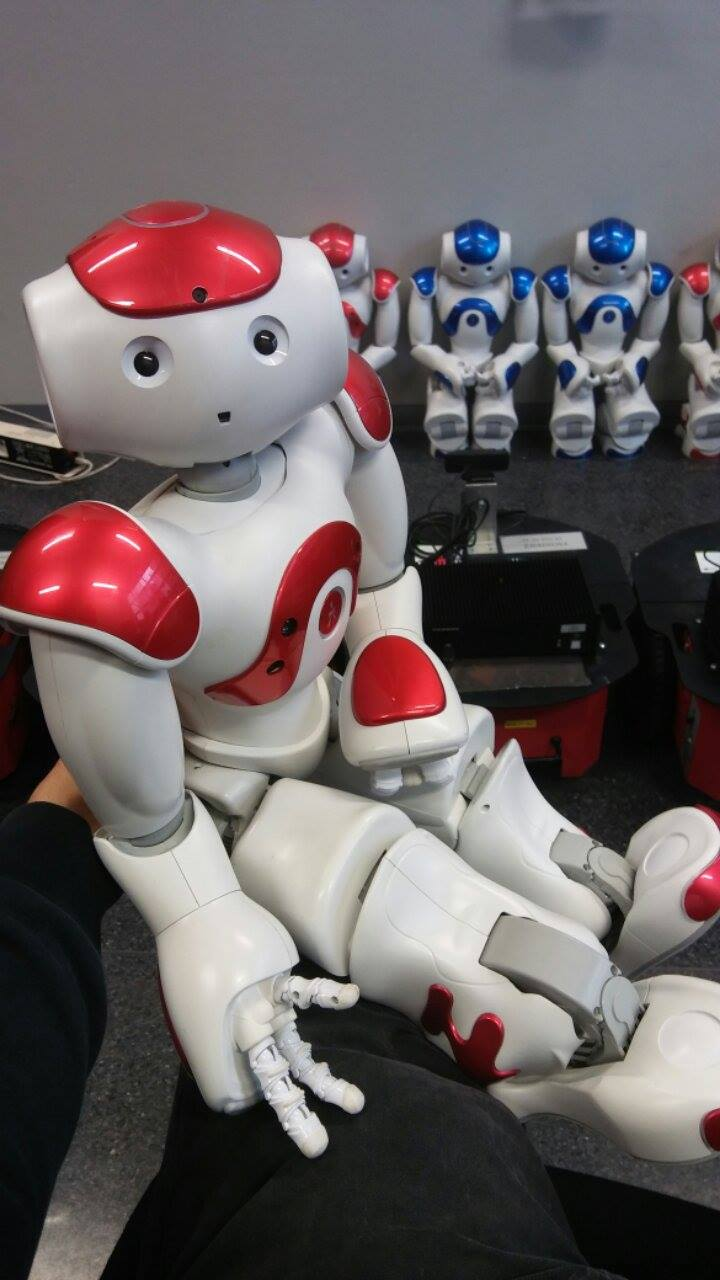
\includegraphics[width=0.35\textwidth]{images/nao.jpg}
    \caption{Robot NAO}
    \label{fig:NAO}
\end{wrapfigure}
Układ sensoryczny przeznaczony do interakcji z człowiekiem obejmuje cztery mikrofony (rejestracja mowy i kierunku przychodzenia dźwięku), kamerę skierowaną do przodu (rozpoznawanie człowieka, twarzy, przedmiotów, etc.), czujniki dotykowe po trzy na dłoniach i na głowie (do wykrywania dotyku dłoni i głowy). Efektory przeznaczone do interakcji z człowiekiem to para głośników (generowanie mowy i innych dźwięków), liczne diody (sygnalizowanie emocji i innych komunikatów niewerbalnych). Platformą sprzętową umysłu NAO jest komputer z procesorem Intel ATOM Z530 1.6~GHz~CPU, pamięcią RAM 1~GB, Flash 2~GB Flash i~kartą pamięci Micro SDHC 8~GB. Platformą programową jest NAOqi, dystrybucja GNU/Linux oparta o Gentoo, dostosowana do sterowania robotami firmy Aldebaran~\cite{NAOqi}.

System operacyjny NAOqi realizuje m.in.: monitorowanie stanu działania robota, komunikację ze zdalnymi czujnikami, udostępnianie zbioru poleceń i funkcji oraz zarządzanie realizowanym scenariuszem. Pod wieloma względami NAOqi pełni podobne funkcje co ROS. Co więcej, NAOqi jest zintegrowana z ROS, co jest nieco szerzej omawiane w rozdziale~\ref{sec:srodowisko}. Producent udostępnia SDK zawierające bogate biblioteki modułów pod Pythona, C++ i Choregraphe. Moduły można zaklasyfikować jako sensory wirtualne (Sensing, Audio, Vision, PeoplePerception), efektory wirtualne (Motions, Trackers, Audio, Leds) oraz komponenty do rozwoju sterownika (System, Communications, Flow Control, Diagnosis, World Representation).
%dające dostęp do wielu kompetencji robota. Z punktu widzenia osoby chcącej zaprogramować scenariusz działania robota można dokonać podziału kompetencji na dwie kategorie: 
%\begin{itemize}
%    \setlength\itemsep{-0.4em}
%    \item niskopoziomową, mechaniczną, związaną z geometrią, dynamiką i czujnikami robota, pozwalającą na przykład na wydawanie komend silnikom, odczyt sygnałów z mikrofonu, kamer lub siłomierzy, czy zmianę koloru diód umieszczonych przy oczach; 
%    \item wysokopoziomową, programową, realizującą zaawansowane algorytmy, takie jak rozpoznanie mowy, lub twarzy, śledzenie obiektu (wodzenie za nim wzrokiem), czy zmianę pozycji i przemieszczenie się do innego miejsca. 
%\end{itemize}

\subsection{NAO jako agent CERT}
\label{subsec:NAOCERT}
Mając na uwadze komponenty główne architektury agenta, omówione w rozdziale~\ref{subsec:CERT}, możemy dokonać przypisania poszczególnych modułów programowych NAOqi API do tych komponentów. 
\begin{description}
\item[perceptory rzeczywiste] Wybrane komponenty z modułów Sensing i Diagnosis które zwracają wartości parametrów mierzonych przez sensory sprzętowe.
\item[perceptory wirtualne] Większość komponentów z modułu Sensing i Audio oraz wszystkie z Vision i PeoplePerception.
\item[efektory wirtualne] Większość komponentów programowych z modułów Motions i Audio, Leds, wszystkie z Trackers.
\item[efektory rzeczywiste] Niektóre komponenty programowe z modułu Motions i Leds (te umożliwiające sterowanie napędami w poszczególnych przegubach i świecenie konkretnymi LED-ami).
\item[sterownik] Audio/Dialog - system dialogowy, Core (System, Flow Control, World Representation) - programowanie i dostęp do zasobów
\item[komunikacja] Communications - przeznaczony do komunikacji pomiędzy agentami osadzonymi w NAO.
\end{description}
%Możemy wspominaną warstwę niskopoziomową potraktować jako receptory i efektory rzeczywiste. Nie pozwalają one bezpośrednio na realizację scenariuszy społecznych, ponieważ nie udostępniają środków do uogólnienia wiedzy, ani nie modelują umysłu. 

%Warstwa wysokopoziomowa będzie traktowana jako wirtualne podsystemy E i R. Znacząco rozszerza możliwości robota, dostarczając wyższych warstw abstrakcji, ułatwiając pracę programiście i pozwalając na interakcję z człowiekiem. Niestety taka interakcja okazuje się płytka i bezosobowa. Dla przykładu robot potrafi śledzić twarz, jednak nie przypisuje jej konkretnej osobie, ponieważ nie ma jak jej rozpoznać i zapamiętać.

\subsection{NAO jako robot społeczny}
Mając na uwadze fakty zebrane w rozdziale~\ref{subsec:NAOCERT} można stwierdzić, że NAO oferuje dobrą bazę dla perceptorów rzeczywistych i wirtualnych oraz efektorów rzeczywistych i wirtualnych. Natomiast z perspektywy modelu BDI agenta, rozważanego w rozdziale~\ref{sec:BDI}, ta podstawa jest dość słaba. NAOqi API nie oferuje bezpośredniego wsparcia dla modelu BDI, nie oferuje również wsparcia dla implementacji sterowników w formie automatu skończonego. Wyżej wymienione modele można zaimplementować, ale startując z nieco niższego poziomu. NAOqi API wspiera paradygmat sterowania behawioralnego (behavior-based control). Ten fakt w połączeniu z uwagami z rodziału~\ref{subsec:robspol} prowadzi do wniosku, że NAO nie spełnia wymogów robota społecznego. Z drugiej strony jest dobrą bazą sprzętowo-programową dla realizacji tego celu.

Powyższy wniosek został sformułowany z perspektywy agenta. Ważna jest również perspektywa użytkownika.
%Za realizację scenariuszy działania odpowiada podsystem sterowania. 
Domyślnie po uruchomieniu, bez ingerencji użytkownika, NAO jest w trybie ,,Autonomus life''.
%jedynie prymitywnym konstruktem cechującym się podstawową responsywnością bazującą na sygnałach odbieranych z wirtualnych receptorów i przekuwanych w odpowiedź przy wykorzystaniu wirtualnych efektorów. 
Jego działania sprowadzają się do przestępowania z nogi na nogę, ruchów przypominających oddech oraz podążaniu wzrokiem za twarzą. To zachowanie jest dość wiarygodne i w krótkiej perspektywie sprawia, że NAO jest postrzegany bardziej jako ożywiony byt niż urządzenie mechatroniczne. W średniej i dłuższej perspektywie zachowanie NAO staje się w przewidywalne i powtarzalne, co powoduje, że zaczyna sprawiać wrażenie zabawki. Generalnie, tworzone dla NAO interaktywne scenariusze zachowań są relatywnie proste i nie są oparte na poważniejszych modelach poznawczych. Między innymi z tego powodu NAO nie jest zdolny do podjęcia wysokopoziomowej interakcji.
%, nie posiada sztucznych emocji, ani nie zapamiętuje osób przebywających w jego otoczeniu, więc nie spełnia wymagań stawianych robotom społecznym.

